%Packages and what they are doing
%\documentclass[10pt]{report}     %settting the type of the document

\documentclass  [
  %paper    = a4, %BCOR     = 10mm, twoside, openright, fontsize = 10pt, toc      = bibnumbered,
  toc      = listofnumbered, numbers  = noendperiod, headings = normal, chapterprefix=true,%my own
  listof   = leveldown, version  = 3.22, bibliography=totoc
]{scrreprt}

\usepackage[utf8]{inputenc}
\usepackage[T1]{fontenc}
\usepackage[english]{babel}   %language and the fontface of the document
\usepackage{amsfonts,amsmath,amssymb} %some math symbols
\usepackage{braket} %for bra's and ket's

%Dummy texts
\usepackage{blindtext}
\usepackage{lipsum}

\usepackage{wrapfig} %creates figures that wrap around text
\usepackage{multicol} %multicolumn text

%Page space settings
%\usepackage{fullpage} %uses the full page
\usepackage[a4paper,bindingoffset=0.2in,%
left=1in,right=1in,top=1in,bottom=1in,%
footskip=.25in]{geometry}

\usepackage[pdftitle={Effects of non-linear excitation on the propagation of light},pdfauthor={Deniz Adigüzel},pdfcreator={},pdfproducer={}]{hyperref}

%------Library settings------
\usepackage[backend=biber, hyperref,url=false, isbn=false, style=alphabetic, sorting=anyt]{biblatex}
\addbibresource{ref.bib}

%_________________________________________________________________________________________

\usepackage{nameref}
\usepackage{todonotes}

\usepackage{mhchem}
\usepackage{soul}


\usepackage{subfiles}

\usepackage{amsmath,amsfonts,amssymb}
\usepackage{physics}
\usepackage{IEEEtrantools}
%\renewcommand{\theequationdis}{{\normalfont (\theequation)}}
%\renewcommand{\theIEEEsubequationdis}{{\normalfont (\theIEEEsubequation)}}
%\renewcommand{\ref}[1]{\eqref{#1}}
\usepackage{cases}
\def\doubleunderline#1{\underline{\underline{#1}}}
\def\doubleoverline#1{\overline{\overline{#1}}}
\newcommand{\vv}[1]{\mathbf{#1}}         %%% vector symbols (std)
\newcommand{\mathcomma}{\,,}  %%% comma in mathematical environment
\usepackage{dsfont}

\usepackage{booktabs}

\usepackage[labelfont=bf,font=small]{caption}
\captionsetup{justification=raggedright,singlelinecheck=false}
\setcapindent{0pt}

\usepackage{adjustbox}
\usepackage{enumitem}
%%\setitemize{wide} % stop wide labels from sticking into margin

\usepackage[normalem]{ulem}


% nice fractions
\usepackage{nicefrac}

% python code
%\usepackage{minted}

% bold mathcal
\DeclareMathAlphabet\mathbfcal{OMS}{cmsy}{b}{n}

% ornaments
\usepackage{fourier-orns}
%\usepackage{fourier}

\usepackage                             {color}
\usepackage                      {graphicx}%[draft]


%---------------------COLORS---------------------
\definecolor{darkblue}{rgb}{0.0,0.0,0.4}
\definecolor{darkgreen}{rgb}{0.0,0.4,0.0}

\hypersetup{
    colorlinks,
    linkcolor=black,
    citecolor=darkgreen,
    urlcolor=darkblue
}
\addtokomafont{disposition}{\rmfamily}

\AtEveryBibitem{%
	\clearfield{month}%
}
 
% increase ToC spacing between number and title
\usepackage{tocloft}
\setlength\cftpartnumwidth{2.5em}
\setlength\cftchapnumwidth{2.5em}
\setlength\cftsecnumwidth{2.5em}
\setlength\cftsubsecnumwidth{3.0em}
\setlength\cftsubsubsecnumwidth{2.5em}

% comments and todo notes
\newcommand{\dl}[1]{{\color{blue}#1}}
\newcommand{\rev}[1]{{\color{red}#1}}

% for moving conclusion chapter out of part
\usepackage{bookmark}


%\usepackage{setspace}
%\usepackage{parskip}
%\usepackage{multirow}
%\usepackage{titlesec}
%usepackage[section]{placeins}
%\usepackage{xcolor}
%\usepackage{breakcites}
%\usepackage{lineno}
%\usepackage{hyphenat}
%\usepackage{etoolbox}
%\usepackage[round]{natbib}
%\usepackage{authblk}
%\usepackage{graphicx}
%\usepackage[space]{grffile}
%\usepackage{latexsym}
%\usepackage{textcomp}
%\usepackage{longtable}
%\usepackage{tabulary}
%\usepackage{booktabs,array,multirow}

\usepackage{verbatim}


\usepackage{dsfont}
\usepackage{MnSymbol}
\usepackage{cleveref}




\setlength{\parindent}{0pt}



\begin{document}
 
\pagenumbering{roman}
  %% title pages similar to providet template instead of maketitle
  %\include{titlepages-ger} % select either german
%% this will generate title pages similar to the template provided
%% by the Department of Physics and Astronomy Heidelberg
%%
%% More information:
%% http://www.physik.uni-heidelberg.de/aktuelles/studium/
%% (PDF link: ...studium/download/145/Vorlage_Diplomarbeit_Formular.pdf)

%% Titleintro
\thispagestyle{empty}
  
\begin{center}
  \renewcommand{\baselinestretch}{2.00}
  \Large\sffamily
  Department of Physics and Astronomy\\
  \large Heidelberg University
  \par\vfill%\normalfont
  Master thesis\\
  in Physics\\
  submitted by\\
  Deniz Adigüzel\\
  born in Istanbul\\
  2026
\end{center}

\newpage
\phantom{thesis}
\thispagestyle{empty}
\cleardoublepage

%% Titlepage
\thispagestyle{empty}
{%\fontfamily{LinuxBiolinumT-OsF}\selectfont
  %\renewcommand{\sfdefault}{LinuxBiolinumT-OsF}
  
\begin{center}

  \renewcommand{\baselinestretch}{2.00}
  %\Large\bfseries\sffamily
    \Large\bfseries%\sffamily
    %(Title)\\
    %(of)\\
    %(Master thesis)
    Propagation effects \\ and theory of Nuclear SAXS
  \\[-1em]
  \line(1,0){250}
  \\
  \normalfont\Large\sffamily
    \large\normalfont 
    %\centering
    %\makebox[1.1\textwidth][c]{
    
 \begin{minipage}{1.1\textwidth}
    %}
    \end{minipage}
    
  
  \par
  
  \vfill
  \large\normalfont
  This Master thesis has been carried out by \\ \textbf{Deniz Adigüzel}\\
  at the\\
  Max Planck Institute for Nuclear Physics\\
  under the supervision of\\
  \textbf{apl. Prof. Dr. J\"org Evers}
  %% additionally insert second supervisor here if carrying out an
  %% external diploma thesis. Reduce vspace in L. 44 accordingly.}
  
 %\end{minipage}
\end{center}\par
%\vspace{1\baselineskip}

% reset baselinestretch
\renewcommand{\baselinestretch}{1.00}\normalsize
}

 % or english title page
  %\renewcommand{\familydefault}{ComputerModern}
  
\null\cleardoublepage

\thispagestyle{plain}
%% Abstract page
%% =============
%%
%% Content of abstract pages has been put into seperate pages to simplify
%% word counting. Use e.g. the unix command
%%   wc abstract-ger.tex
%% or
%%   wc abstract-eng.tex
%% to get the number of words contained in these files.
\thispagestyle{empty}
%\begin{center}
  \noindent\sffamily\textbf{Abstract}
	\\[1em]\normalfont\normalsize

With the increasing number of nuclear-resonant photons per pulse at x-ray free electron lasers (XFELs) \cite{scientific_opp_XFEL}, achieving higher excitation levels experimentally becomes feasible \cite{Shvydko2023}. This development makes it particularly compelling to investigate light propagation and dynamics beyond the low-excitation regime (LER) and around population inversion. Thus, in this thesis, we examine the time response of resonant nuclear scattering of x-rays beyond the LER. In the LER, it is possible to obtain an analytical solution for light propagation, which becomes not possible beyond this regime. To study dynamics beyond the LER, we employ numerical methods to analyze propagation effects and nuclear dynamics. We implement the method of lines (MOL) to solve the Maxwell-Bloch equations.\\

First, we compare our results with those of Wolff \cite{wolff2023characterization} in the LER using thin targets, where the effects arising from the propagation of light through the target can be neglected. We generalize their results by analyzing the dynamics in thick targets, considering the propagation effects. Subsequently, we extend our investigation beyond the LER to the regime of population inversion and beyond. Here, we discover interesting phenomena, such as time shifts in the minima of the observed coherently scattered light intensity and transitions around population inversions. We propose an experimental signature to detect nonlinear excitations by calculating the relative time shifts as a function of target thickness. Finally, we analyze our model in the non-decaying limit ($\gamma = 0$) and find good agreement with the results from Burnham and Chiao \cite{BURNHAM1969}, concluding that spontaneous decay plays a major role in the creation of transitions around population inversions.


  \vfill
  \vspace{1cm}
  %\begin{minipage}[c][0.48\textheight][b]{0.9\textwidth}
    %\small
    %\textbf{
    %  
    %}\par
    %\vspace{\baselineskip}
    %\normalfont\normalsize
    \noindent\sffamily\textbf{Abstrakt}
	\\[1em]\normalfont\normalsize
Mit der zunehmenden Anzahl von nuklear-resonanten Photonen pro Puls beim XFELs \cite{scientific_opp_XFEL} wird es experimentell möglich, höhere Anregungsniveaus zu erreichen \cite{Shvydko2023}. Diese Entwicklung macht es besonders interessant, die Lichtausbreitung und Dynamik über das Niedriganregungsregime (LER) hinaus sowie um die Populationsinversion zu untersuchen. In dieser Arbeit analysieren wir daher das Zeitverhalten der resonanten nuklearen Streuung von Röntgenstrahlen außerhalb des LER. Im LER ist es möglich, eine analytische Lösung für die Lichtausbreitung zu erhalten, was in höheren Anregungsbereichen nicht mehr möglich ist. Um die Dynamik in diesen höheren Bereichen zu untersuchen, verwenden wir numerische Methoden, um die Ausbreitungseffekte und die Kerndynamik zu analysieren. Wir implementieren die Methode der Linien (MOL), um die Maxwell-Bloch-Gleichungen zu lösen.\\

Zunächst vergleichen wir unsere Ergebnisse mit denen von Wolff \cite{wolff2023characterization} im LER unter Verwendung dünner Targets, bei denen die durch die Lichtausbreitung im Target entstehenden Effekte vernachlässigt werden können. Wir erweitern deren Ergebnisse, indem wir die Dynamik in dicken Targets unter Berücksichtigung der Ausbreitungseffekte analysieren. Anschließend untersuchen wir den Bereich der Populationsinversion und darüber hinaus. Hier entdecken wir interessante Phänomene wie Zeitverschiebungen in den Minima der beobachteten kohärent gestreuten Lichtintensität und Übergänge um die Populationsinversionen. Wir schlagen eine experimentelle Signatur vor, um nichtlineare Anregungen durch Berechnung der relativen Zeitverschiebungen in Abhängigkeit von der Targetdicke zu detektieren. Schließlich analysieren wir unser Modell im nicht zerfallenden Grenzfall ($\gamma = 0$) und finden eine gute Übereinstimmung mit den Ergebnissen von Burnham und Chiao \cite{BURNHAM1969}. Wir kommen zu dem Schluss, dass der spontane Zerfall eine wesentliche Rolle bei der Entstehung der Übergänge um die Populationsinversionen spielt.
    %\input{abstract-eng}
  %\end{minipage}
%\end{center}

\thispagestyle{empty}

    %\listoftodos

  \tableofcontents
  
 \null\cleardoublepage
  
  \pagenumbering{arabic} %% start page 1
  \pagestyle{headings}
%  \pagestyle{fancy}
  \setcounter{page}{1}

\chapter{Introduction}

\section{Motivation}
The investigation and manipulation of quantum systems are crucial for various applications and technological advancements, as well as for addressing fundamental research questions in physics. In recent years experiments progressed rapidly and we are seeing new technologies emerge in quantum science \cite{QS_1,QS_2} such as quantum computers \cite{quantumcomp1, quantumcomp2}, quantum simulators \cite{quantumsimulators1} and much more.\\

Here quantum optics is such a branch of quantum systems which explores the fundamental interactions between light and matter at the quantum level. It delves into phenomena such as photon entanglement, quantum coherence, and the manipulation of quantum states of light. The study of quantum optics has led to groundbreaking advancements in quantum computing, secure communication \cite{quantuminformation}, and precision measurement technologies \cite{Heeg2017}.\\

Central to quantum optics is the understanding of how light interacts with atomic and molecular systems. These interactions are characterized by phenomena such as spontaneous and stimulated emission, absorption, and scattering, all of which are governed by the principles of quantum mechanics. Relatively new, the field has expanded to encompass X-ray quantum optics, where similar principles are applied to much shorter wavelengths \cite{scientific_opp_XFEL}. X-ray photons, with their higher energies, provide unique opportunities to probe matter with atomic-scale resolution and to explore new regimes of light-matter interaction. X-ray quantum optics opens up possibilities for investigating phenomena such as quantum control of excitons \cite{Heeg2021}, and the development of novel spectroscopic techniques.\\

One of the most intriguing intersections of quantum optics and X-ray physics is found in the study of the Mössbauer effect. The Mössbauer effect, discovered by Rudolf Mössbauer in 1958 \cite{Mssbauer1958}, involves the recoil-free emission and absorption of gamma rays by atomic nuclei bound in a solid. Due to the narrow linewidth of Mössbauer nuclei, this effect provides a highly precise method for examining hyperfine interactions and allows for the study of extremely narrow spectral lines, which are invaluable in various scientific applications such as in materials science, chemistry, and biology. Other than the x-ray quantum optics, Mössbauer effect finds its way in other very diverse areas, such as archaeology \cite{Wagner2004_archeology}, battery development \cite{Lippens2021_battery} and more recently, planetary exploration with a Mössbauer spectrometer sent to Mars on the Mars Exploration Rover to search for water \cite{Klingelhofer2004_mars}.\\

Moreover, in nuclear quantum optics \cite{Adams2013}, many optical schemes have been successfully adapted to the x-ray regime, including Lamb shift \cite{collectivelambshift}, superradiance \cite{superradiance}, electromagnetically induced transparency \cite{EITinxray}, spontaneously generated coherences \cite{spontaneouslygeneratedcoherences}, among others. \\

The main limiting factor in nuclear quantum optics is the current light sources, such as PETRA \MakeUppercase{\romannumeral 3} at DESY in Hamburg \cite{desy} or ESRF in Grenoble \cite{esrf}, which can deliver on average less than one resonant photon per pulse due to the narrow linewidth. As a result, experiments on Mössbauer nuclei have been restricted to low-excitation regime (LER) so far. Attempts to achieve higher excitations and nuclear inversion was a long standing dream \cite{oldproblem1,oldproblem2,oldproblem3}.   \\

However, with self seeded x-ray free electron lasers (XFEL) \cite{xrayFEL, XFEL2} in the hard x-ray regime, a significant improvement of the number of nuclear-resonant photons per pulse on average \cite{Shvydko2023,superradiance} can be achieved. Additionally, by utilizing advanced measuring schemes and improved focusing techniques \cite{dominik_higherexcitation}, achieving higher excitations beyond the low-excitation regime is becoming increasingly feasible.\\

Theoretically, the interaction between light and matter is described by the Maxwell-Bloch equations. In general, it is not possible to solve the Maxwell-Bloch equations analytically. Nevertheless under certain conditions analytical results can be obtained. For example, in the low-excitation regime these equation can be solved to obtain the \textit{response function}, a well-established technique to describe the nuclear dynamics \cite{Rhlsberger2005}. This attempt can be expended with a perturbation approach as in \cite{wolff2023characterization}. In this work they derived a ratio between the coherent and incoherent light that remains constant over time within the LER but varies beyond it, which then can be used to evaluate the regime that one operates the experiment. This is an important tool to differentiate the different levels of excitations, especially in the time where due to the x-ray free electron lasers more and more resonant photons per pulse can be generated. The main results of this work are shown in \Cref{fig:lukas_result}. However, they did not take into account the effects resulting from propagation of light through thick targets. \\

Another possibility to solve the Maxwell-Bloch equations analytically is to consider the times much shorter compared to the characteristic decay of the excited states \cite{BURNHAM1969}. Burnham et.al. developed a model that approximates the light propagation and nuclear dynamics in an excitation regime from the LER to population inversion. \\
\begin{figure}
    \centering
    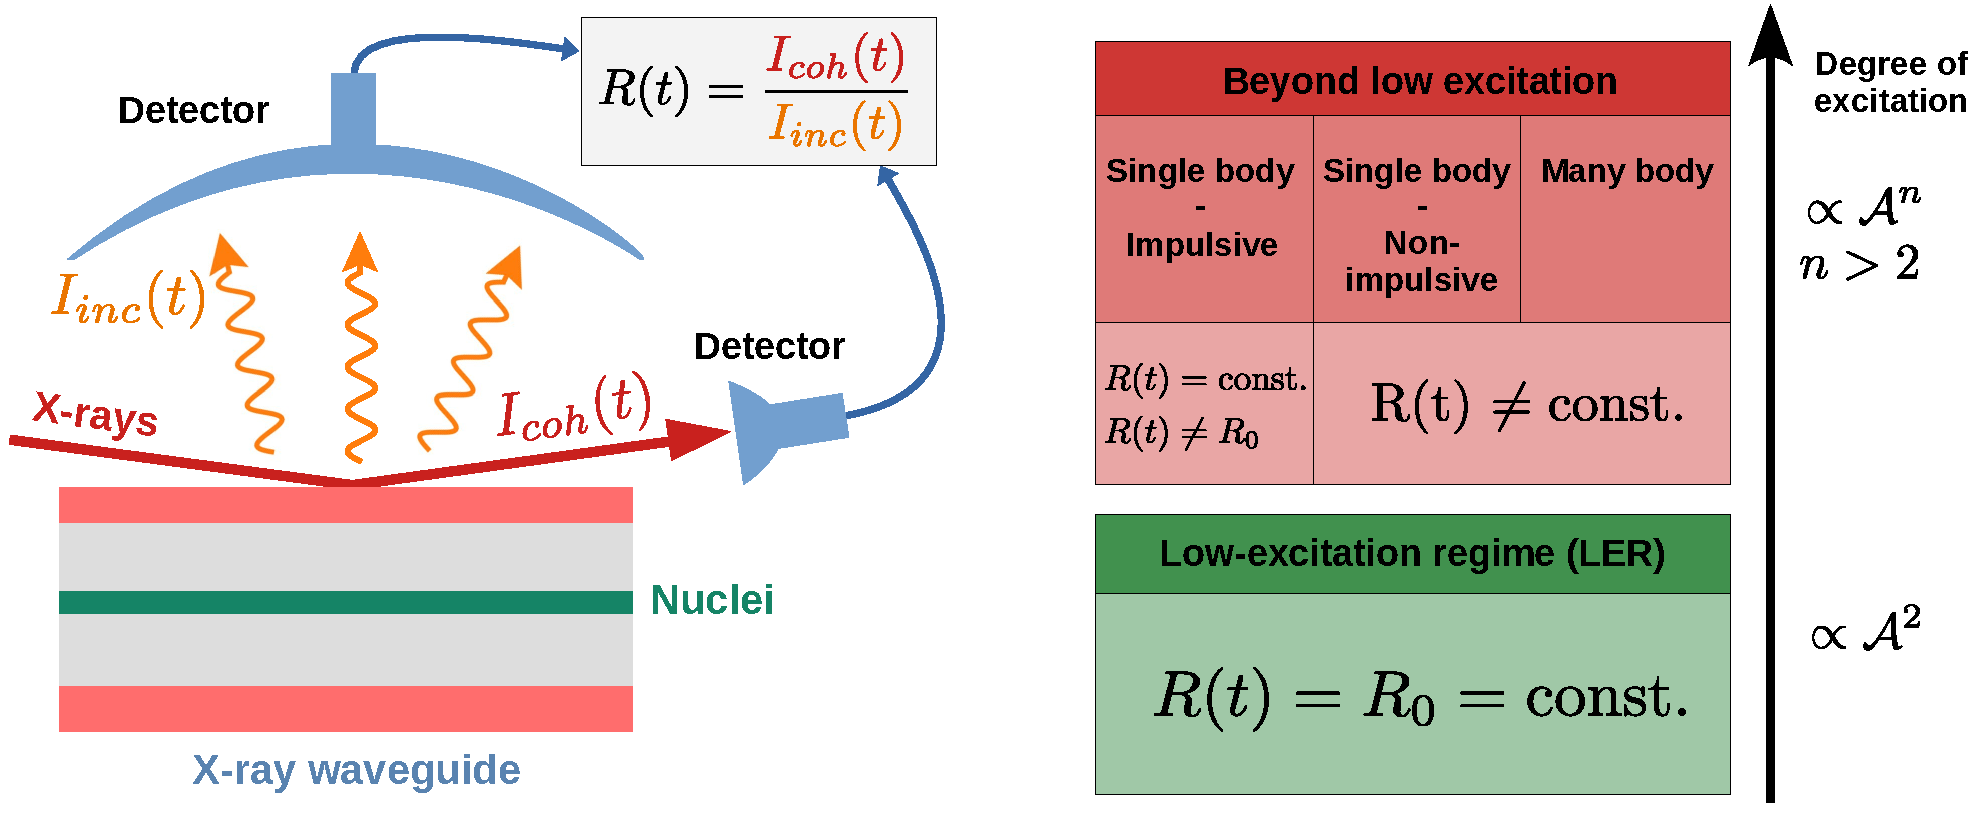
\includegraphics[width =0.75\textwidth]{data/introduction/OverviewPicture.pdf}
    \caption{Characterization and detection method for x-ray excitation beyond the low-excitation regime. Here the main results are displayed from \cite{wolff2023characterization}. In this work, they were able to show that the ratio of coherent to incoherent light stays constant over time in the low excitation regime. For coherent light $I_\mathrm{coh} = |\rho_{eg}|^2$ and for incoherent light $I_\mathrm{inc} = \rho_{ee}$ was used, as there were no propagation effects taken into account. (This figure is reproduced with the permission of the authors \cite{wolff2023characterization}.)} 
    \label{fig:lukas_result}
\end{figure}


\section{Goals of this thesis}

In this thesis, we want to extend the previous works in two directions which can be seen in \cref{fig:model_comp}. First, we want to analyse stronger excitations even beyond inversion and secondly we want to include propagation effects in thicker targets. Our objectives include comparing the dynamics within the low excitation regime (LER) under without propagation effects with the results presented in \cite{wolff2023characterization} and extend the analysis to thicker targets, where propagation effects have to be taken into account. Subsequently, we want to investigate dynamics beyond the low excitation regime under the non-decaying limit ($\gamma = 0$) and compare our results with those of \cite{BURNHAM1969}. Additionally, we will explore the decaying limit beyond the low excitation regime and population inversion, uncovering interesting structures. Finally, we will propose an experimental signature capable of detecting nonlinear excitation through the time shifts of intensity minima.\\

\begin{figure}
    \centering
    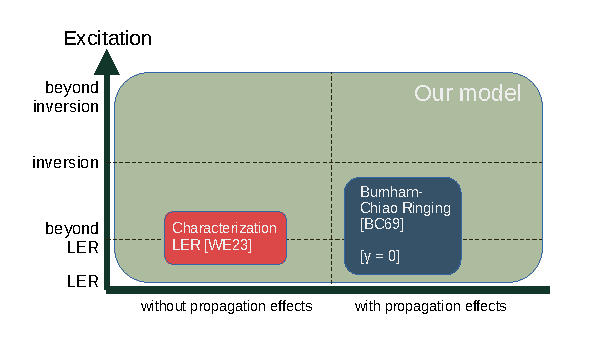
\includegraphics[width = 0.85\textwidth]{data/introduction/resultsvergleich_2.pdf}
    \caption{An overview is given to compare the limits of different models. \cite{wolff2023characterization} proposes methods to characterize the low-excitation regime without taking into account the propagation effects. On the other hand, \cite{BURNHAM1969} gives a model that approximates the dynamics from LER to population inversion in the non-decaying limit. With our model, we can analyse the low excitation regime as well as higher excitations and beyond the population with propagation effects and spontaneous decay.}
    \label{fig:model_comp}
\end{figure}


\section{Thesis outline}

In Chapter 2, an introduction will be provided to quantum optical two-level systems and light-matter interactions. The Maxwell-Bloch equations will be presented, and the response function formalism in the time domain will be derived. Additionally, the results from Burnham and Chiao \cite{BURNHAM1969} will be summarized. In Chapter 3, the method of lines will be introduced. This method will be used to discretize the spatial component of the Maxwell-Bloch equations. Consequently, this discretization will enable us to solve coupled ordinary differential equations instead of a partial differential equation. In Chapter 4, we will present our results. The first half focuses on the Low Excitation Regime (LER), where we compare our findings with those of \cite{wolff2023characterization} and extend them to include the propagation limit. The second half delves into dynamics beyond the LER and population inversion, where we compare our results under the non-decaying limit and generalize to the decaying limit. In Chapter 5, a summary of the findings will be presented, highlighting key insights and conclusions drawn from the study. Additionally, an outlook will be provided, discussing the applicability of the developed model in other settings.

\chapter{Theoretical Background}
In this chapter, the equations of motion (EOM) for nuclear forward scattering (NFS) will be derived semiclassically, such as the response function formalism in the low excitation regime. We start with an introduction to quantum optics and two level systems. We will then extend this to the open quantum systems formalism, to be able to integrate the spontaneous emission to our model. Doing so, we arrive at the optical-bloch equations. Response function in time domain will be derived by fourier transforming the frequency-domain solution of the optical Bloch equations to the time domain. \\\
\begin{figure}[b!]
    \centering
    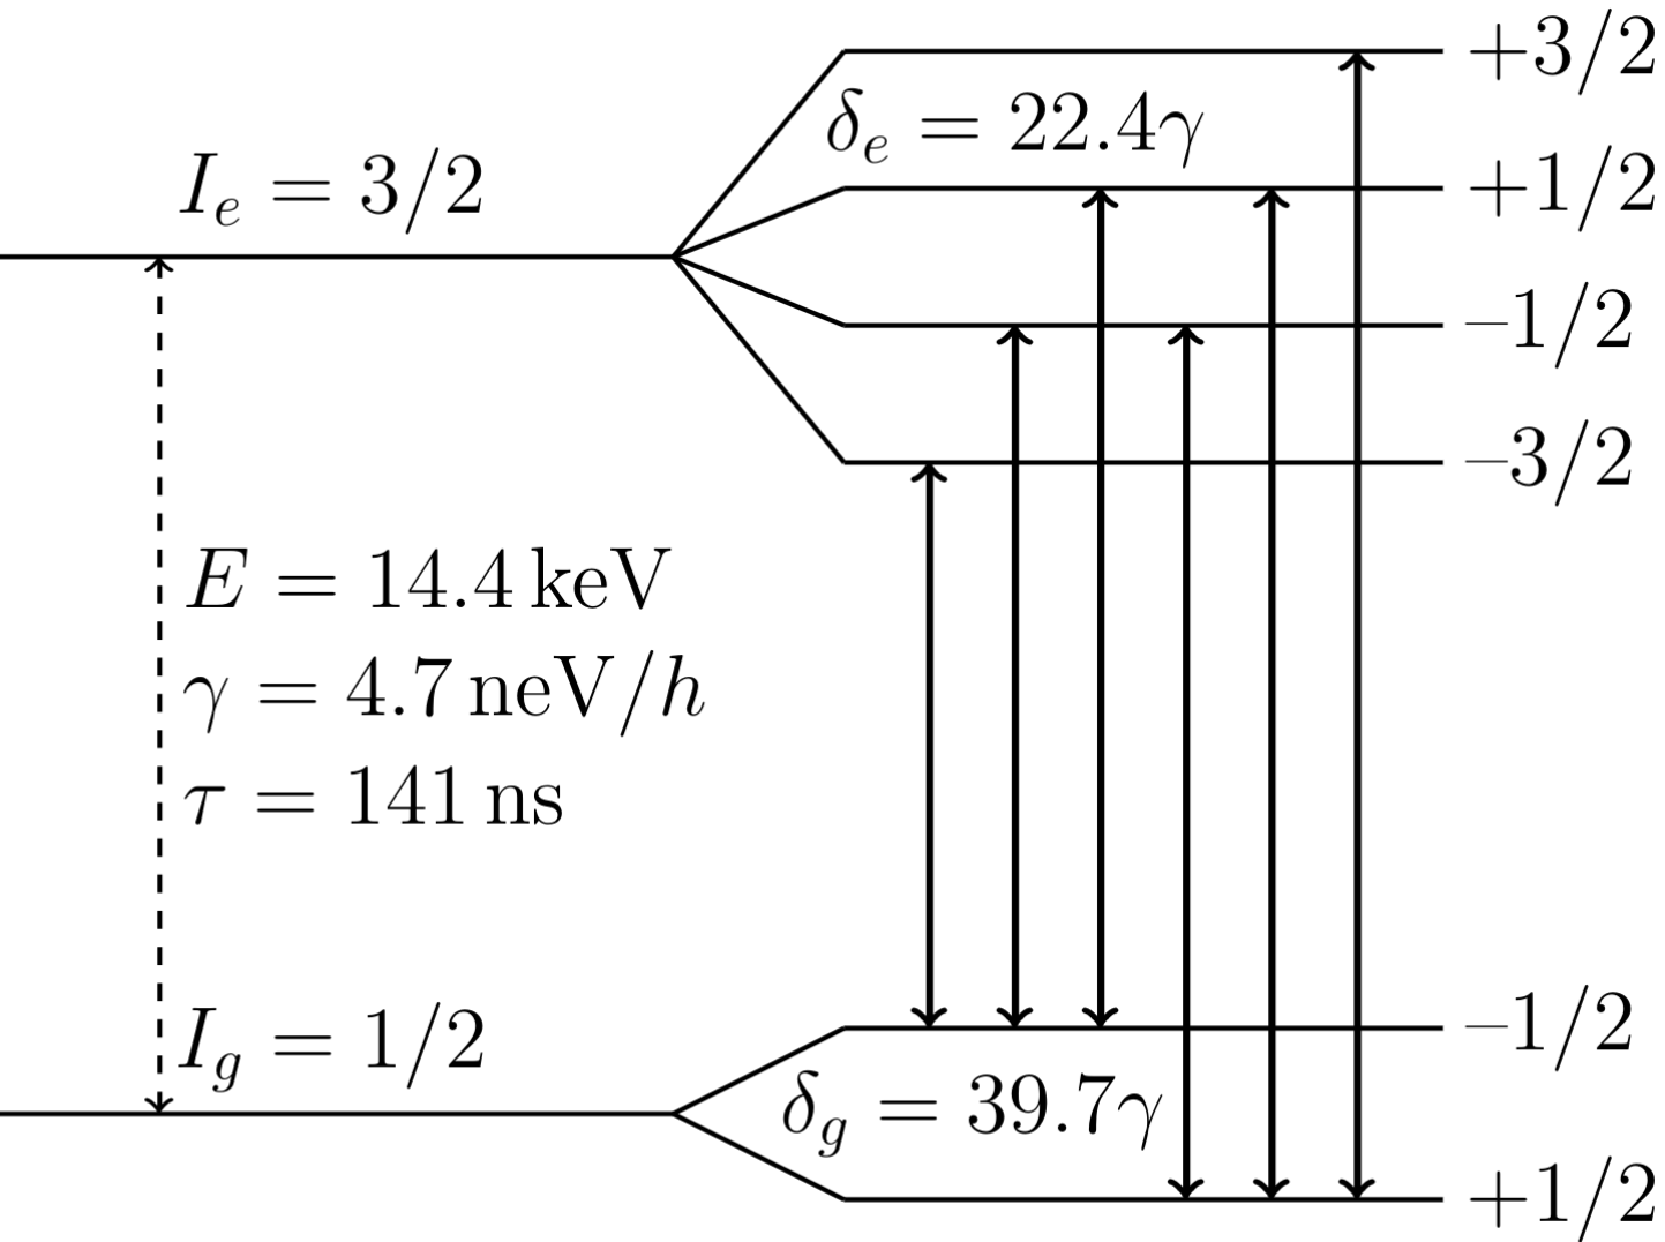
\includegraphics[width = 0.5\textwidth]{data/background/mossbauer_transitions2.pdf}
    \caption{ Mössbauer transitions in $\ce{^{57}_{}Fe} $. Here $I_g$ and $I_e$ denotes the nuclear spins of the ground and excited state, respectively, $E$ the transition energy, $\gamma$ the linewidth, $\tau$ natural lifetime. In the presence of a magnetic hyperfine field, two states split up to 6 states.(Adapted from \cite{https://doi.org/10.11588/heidok.00017869})}
    \label{fig:mossbauertransitions}
\end{figure}

\section{Mössbauer}




\subsection{Mössbauer isotopes as an extreme platform for quantum optics}
The Mössbauer effect was found by Rudolf L. Mössbauer in 1958 \cite{Mssbauer1958}, for which he received a Nobel prize in 1961. In this effect the momenta of the photons are absorbed by the entire lattice without phonon creation/annihilation, which enables the recoil-free absorption and emission of photons. Due to the recoil-free absorption, the linewidth of these transitions are extremely narrow, which makes them a perfect candidate for precision spectroscopy \cite{2012rudolfmossbauerstory, Rhlsberger2005}. \\

In \Cref{fig:mossbauertransitions}, the relevant nuclear transitions of $\ce{^{57}_{}Fe} $ can be seen. The isotope $\ce{^{57}_{}Fe} $ is the most widely used Mössbauer isotope \cite{Heeg2021}, but other isotopes are also being used, e.g. scandium \cite{Shvydko2023}. A complete list of Mössbauer nuclei can be found in the appendix of \cite{Rhlsberger2005}.\\

Besides the extremely narrow linewidths Mössbauer nuclei prove, they are mostly in the hard x-ray regime, with transition energies around and above 10 keV. Due to the extremely narrow linewidths, it was not possible to reach high excitations \cite{oldproblem1,oldproblem2,oldproblem3}. With the advancement of seeded x-ray free electron lasers in hard x-ray regime and novel measuring schemes, it is possible to generate more nuclear-resonant photons \cite{McNeil2010,RevModPhys.88.015006}. First experiments have already proven the advantage of the orders of magnitude higher photon flux as compared to synchrotrons \cite{Rffer2021,Shvydko2023}. \\

\subsection{Nuclear forward scattering}
To investigate the structure and dynamics of condensed matter, one of the most powerful methods is the scattering of x-rays, such as: Diffraction, Spectroscopy and Imaging. An example setup of such a nuclear forward scattering experiment at XFELs can be seen in \Cref{fig:NFS_setup}. Here incident x-ray pulse excites the nuclei in the sample. These excited nuclei would then undergo spontaneous emission, where they emit position and time dependent radiation. A coherent superposition of emitted lights would then interfere, which results in a characteristic spectrum as a time response \cite{Rhlsberger2005}.  

\begin{figure}
    \centering
    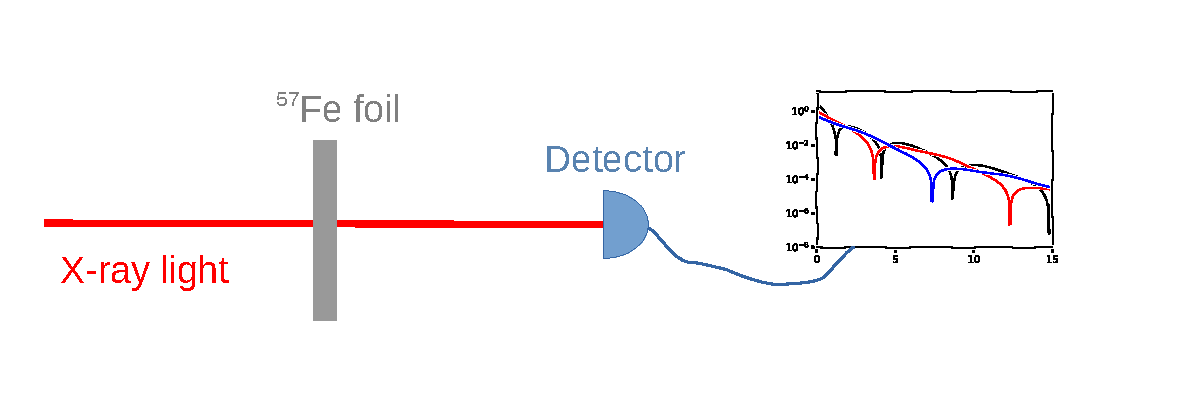
\includegraphics[width = 1\textwidth]{data/background/setup_2.pdf}
    \caption{Setup of the nuclear forward scattering experiment. The x-ray light is scattered and the coherent light can be measured in the direction of the incident light, as it is highly directional. (Adapted from M. Gerharz Poster.)}
    \label{fig:NFS_setup}
\end{figure}


\subsection{Calculation of b parameter to physical thickness}
In theory, a theoretical thickness parameter $b$ is used to describe the physical thickness of the target $d$. This $b$ parameter can be expressed in terms of material properties by \cite{https://doi.org/10.11588/heidok.00017869, lentrodt2021ab, wolff2023detecting} as
\begin{equation}
    \mathrm{b} = \frac{\pi \rho}{2 k_0^2} \frac{f_{\mathrm{LM}}}{(1+\alpha)} \frac{2I_{e} +1}{2 I_{g}+1} \gamma \mathrm{d}\, , \label{b_phys}
\end{equation}

where for $\alpha$-iron ($\ce{^{57}_{}Fe} $),  $\rho = 83.13 \;\mathrm{nm}^{-3}$ is the nuclear density, $k_0 = 73.039 \;\mathrm{nm}^{-1}$ the wave vector of the transition, $f_\mathrm{LM} \approx 0.8$ the Lamb-Mössbauer factor, $\alpha = 8.56$ the factor of internal conversion, $I_e = 3/2$, $I_g = 1/2$ the spins of the nuclear excited and ground states, respectively, $\gamma = 4.66 \; \mathrm{neV}$ is the natural linewidth of the resonance. Plugging these values in \Cref{b_phys}, we receive a conversion factor
\begin{equation}
    d = 0.249 \;\; \mu \mathrm{m} \cdot \mathrm{b}[\gamma]\label{b_conversion}\, .
\end{equation}

%%%%%%%%%%%%%%%%%%%%%%%%%%%%%%%%%%%%%%%%%%%%%%%%%%%%%%%%%%%%%%%%%%%%%%%%%%%%%%%%%%%%%%%%%%%%%%%%%%%%%%%%%%%%%%%%%%%%%%%%%%%%%%%%%%%%%%%%%%%%%%%%%


\section{Quantum optical model}

\subsection{Light-Matter Interaction}

The interaction between a radiation field and matter can be calculated, where the matter is modelled as a two level system. Here we use a basis of $\{\ket{g}, \ket{e}\}$, denoting ground and excited states, correspondingly. Furthermore, these two states have an energy difference of $\Delta E_{12} = \hbar (\omega_2 - \omega_1) = \hbar \omega_0$, where in the last equality we just denote the energy difference of these states as the transition energy $\hbar \omega_0$. The Hamiltonian of this system is given as \cite{bloch2004licht}:
\begin{equation} \label{timehamiltonian}
    H = H_{\textrm{atom}} + V = \hbar \omega_0 \ket{e} \bra{e} - \hat{d} \Vec{E}(t) \, . 
\end{equation}
Here the first term is the energy of the excited state and the second term is the light matter interaction operator, given in the \textbf{dipole approximation}, meaning that the electric field is position independent. The operator $\hat{d}$ is the electric dipole-operator and is given by: $\hat{d} = -e \hat{\Vec{r}}$. The electric field can be written as \cite{Scully_Zubairy_1997, reiser2014time}:

\begin{equation}
    \Vec{E}(t) = \frac{E_0}{2} \;  e^{-i\nu t + i \phi(t) + ikz} + \;\; \textrm{c.c.}\, ,
\end{equation}
where $E_0$ is the amplitude, $\nu $ the carrier frequency of light field, k the wavevector and $\phi(t)$ the phase of the incident light field. In \textbf{Rotating wave approximation}, the Hamiltonian in (\ref{timehamiltonian}) can be written as \cite{bloch2004licht}:
\begin{equation} \label{thehamiltonian}
    H = \hbar \omega_0 \ket{e} \bra{e} - \frac{\hbar}{2} \Omega(t) e^{-i(\omega_0 + \Delta)t + i\phi(t)} \ket{e}\bra{g}
    -\frac{\hbar}{2} \Omega^*(t) e^{-i(\omega_0 + \Delta)t - i\phi(t)} \ket{g}\bra{e} \, ,
\end{equation}
where we introduced the detuning $\Delta = \nu - \omega_0 $. The coupling is quantified by the Rabi-frequency:
\begin{equation}
    \Omega(t) = \frac{d_{eg}}{\hbar} E_0(t) \; . \label{rabi_omega}
\end{equation}
Here $d_{eg} $ denotes the dipole matrix element and $\hbar$ the Planck's constant. 


\subsection{Spontaneous Emission}
In experiments, we often have to consider open quantum systems and thus need to include spontaneous emission into our description of the light-atom interaction. Spontaneous emission destroys coherence and for that cannot be described by pure states. Those mixed states can be described with the density matrix formalism.\\

A density matrix $\rho(t)= \ket{\Psi} \bra{\Psi}$ describes the quantum state $\ket{\Psi(t)}$ at time t. The dynamics of the density matrix are governed by the \textbf{Master Equation}
\begin{equation} \label{master_eq}
    \frac{d}{dt} \hat{\rho} = \frac{1}{i\hbar} \left[\hat{H}, \hat{\rho}   \right] + \mathcal{L}[\hat{\rho}] \, .
\end{equation}

Here $\left[\hat{A},\hat{B}\right] = \hat{A} \cdot\hat{B} - \hat{B} \cdot\hat{A}$ denotes the commutator and describes the unitary dynamics of the system. The second term is called the \textbf{Lindbladian} and describes the non-unitary and incoherent dynamics of the system, which can be written as
\begin{equation}\label{lindbladian}
    \mathcal{L}[\hat{\rho}] = -\frac{\gamma}{2} (\sigma^+ \sigma^- \hat{\rho} +\hat{\rho}\sigma^+ \sigma^- -2\sigma^- \hat{\rho}\sigma^+  )\,.
\end{equation}
The operators $\sigma^+$ and $\sigma^-$ are ladder operators and are given by $\sigma^+ = \ket{e}\bra{g}$ and  $\sigma^- = \ket{g}\bra{e}$, $\gamma$ is the rate of spontaneous emission. Another important property of the two level system is that the trace of the density matrix equals to 1:
\begin{equation}
    \mathrm{Tr}[\rho] = 1 \;\;\;\;\;\longrightarrow\;\;\;\;\; \rho_{gg} + \rho_{ee} = 1\, .
\end{equation}

\subsection{Maxwell-Bloch Equations}
Using the Master Equation (\ref{master_eq}) with the Lindbladian (\ref{lindbladian}), we can calculate the density matrix of the two level system $\rho_{ij} = \bra{i} \hat{\rho} \ket{j}$. This set of equations is called the \textbf{Optical Bloch equations} \cite{bloch2004licht, reiser2014time}:
\begin{subequations}
\begin{align}
    \dot{\rho}_{ee} &= -\gamma \rho_{ee} + i \frac{\Omega(t)}{2} e^{-i \nu t + i \phi(t)} \rho_{ge} - i \frac{\Omega^*(t)}{2} e^{+i \nu t - i \phi(t)} \rho_{eg} \, ,\\
    \dot{\rho}_{gg} &= +\gamma \rho_{ee} - i \frac{\Omega(t)}{2} e^{-i \nu t + i \phi(t)} \rho_{ge} + i \frac{\Omega^*(t)}{2} e^{+i \nu t - i \phi(t)} \rho_{eg} \, ,\\
    \dot{\rho}_{eg} &= - \frac{\gamma}{2} \rho_{eg} - i \omega_0 \rho_{eg} + i \frac{\Omega(t)}{2} e^{-i \nu t + i \phi(t)} \rho_{gg} - i \frac{\Omega^*(t)}{2} e^{+i \nu t - i \phi(t)} \rho_{ee}\, , \\
    \rho_{eg} &= \rho^*_{ge}\, .
\end{align}
\end{subequations}
Here $\rho_{ee}$ denotes the density matrix element of atom being in the excited state $\ket{e}$, $\rho_{gg}$ denotes the atom being in the ground state $\ket{g}$ and $\rho_{eg}$ denotes the density matrix element corresponding to the coherence between the ground state $\ket{g}$ and the excited state $\ket{e}$ induced by the propagating field. Using an interaction picture in the form $\Tilde{\rho}_{ge} = \rho_{ge}\; e^{-i(\omega_0 + \Delta)t + i\phi(t)}$, the optical bloch equations simplify to \cite{Scully_Zubairy_1997, reiser2014time}:
\begin{subequations}
\begin{align}
    \dot{\rho}_{ee} &= -\gamma \rho_{ee} + i \frac{\Omega(t)}{2} \Tilde{\rho}_{ge} - i \frac{\Omega^*(t)}{2} \Tilde{\rho}_{eg}\, , \label{rhoee} \\
    \dot{\rho}_{gg} &= +\gamma \rho_{ee} - i \frac{\Omega(t)}{2} \Tilde{\rho}_{ge} + i \frac{\Omega^*(t)}{2} \Tilde{\rho}_{eg}\, ,\label{rhogg} \\
    \dot{\rho}_{eg} &= \left( -\frac{\gamma}{2} + i\Delta -i\dot{\phi}(t) \right) \Tilde{\rho}_{eg} + i\frac{\Omega(t)}{2} \rho_{gg} - i\frac{\Omega^*(t)}{2} \rho_{ee} \label{rhoeg}\, , \\
    \rho_{eg} &= \rho^*_{ge}\, . \label{rhoge}
\end{align}
\end{subequations}
In the next step, we want to calculate the propagation of light in a medium which is modeled by a two level system, like in equations (\ref{rhoee})-(\ref{rhoge}). The propagation of such an electric field is governed by Maxwell's equations. In the semiclassical theory, the polarisation depends on the density matrix element. Using the \textit{slowly-varying envelope approximation}, we get a coupled differential equation for the Wave Equation \cite{PhysRevA.76.033817,Scully_Zubairy_1997,reiser2014time}:
\begin{equation} \label{waveeq}
    \left(\frac{\partial}{\partial z} + \frac{1}{c_0} \frac{\partial}{\partial t} \right) \Omega_0+  \Omega_0\left(\frac{\partial}{\partial z} + \frac{1}{c_0} \frac{\partial}{\partial t} \right) \left(i\phi(t,z) \right) = i\eta \Tilde{\rho}_{eg}
\end{equation}
Here $\eta$ is the coupling parameter between $\Omega$ and $\rho_{eg}$. The Equations (\ref{rhoee})-(\ref{rhoge}) and \Cref{waveeq} are called the Maxwell-Bloch Equations and are the main set of equations, which will be used throughout this thesis. For our discussion, we set the additional phase of the incident light field to zero $\phi(t) = 0$ for simplicity. 

\subsection{Pulse area theorem}\label{section:pulseareatheorem}
Consider a non-decaying two-level system driven by a resonant field. Assuming the system to be initially in the ground state, i.e.$\;\rho_{gg} = 1$, the excited state population can be calculated with the \textbf{area theorem} \cite{allen1987optical, meystre2007elements}:
\begin{subequations}
\begin{align}
    \rho_{ee}(t) &= \sin^2[\mathcal{A}(t)] \label{pulse_area_theorem_rhoee}\, ,\\
    \rho_{ge}(t) &= - \frac{i}{2} e^{i\phi} \sin[\mathcal{A}(t)] \label{pulse_area_theorem_rhoge}\, .
\end{align}
\end{subequations}
Here t denotes the passed time after the incident light pulse. The pulse area is calculated by
\begin{equation}
    \mathcal{A}(t) = \int_{t_0}^t |\Omega(t^\prime)| \mathrm{d}t^\prime\, , 
\end{equation}
where $\Omega(t)$ denotes the Rabi frequency, which is proportional to incident light packet in \cref{rabi_omega}.
%%%%%%%%%%%%%%%%%%%%%%%%%%%%%%%%%%%%%%%%%%%%%%%%%%%%%%%%%%%%%%%%%%%%%%%%%%%%%%%%%%%%%%%%%%%%%%%%%%%%%%%%%%%%%%%%%%%%%%%%%%

\section{Low excitation regime}
The excitation of the nuclei varies depending on the pulse area of the incident light. Two significant regimes are distinguished: the low excitation regime, where most of the nuclei are in the ground state and can be approximated by the low excitation approximation, and the population inversion regime, where all the nuclei are in the excited state ($\rho_{ee} = 1$). An important characterization method for distinguishing between these regimes is outlined in \cite{wolff2023characterization}. This paper presents methods that can effectively differentiate between the low excitation regime and states beyond it.\\

\subsection{Low Excitation Approximation}
Despite the potential for higher numbers of resonant photons per pulse promised by new x-ray free electron lasers, experiments on Mössbauer nuclei have thus far been limited to the low excitation regime due to the small number of resonant photons available. Consequently, we assume the pulse area to be very small, denoted as $\mathcal{A} \ll \pi$, leading to what is commonly referred to as the linear approximation:

\begin{equation}
\rho_{gg} \approx 1 \quad \longrightarrow \quad \rho_{ee} \approx 0 \, .
\end{equation}

Here, $\rho_{gg}$ represents the population of nuclei in the ground state, while $\rho_{ee}$ represents the population of nuclei in the excited state. This approximation assumes that the majority of nuclei remain in the ground state.\\

\subsection{Response function in time and frequency domain}\label{section_respfunction}
The Maxwell-Bloch equations are a set of coupled partial differential equations and in general can't be solved analytically. However, in the low excitation approximation the Maxwell-Bloch equations decouples and can be solved analytically. In this case, the equations (\ref{rhoee})-(\ref{rhoge}) and \Cref{waveeq} reduce to
\begin{align}
    \dot{\rho}_{eg} &= -\frac{\gamma}{2} \Tilde{\rho}_{eg} + i\Delta \Tilde{\rho}_{eg} + \frac{i}{2} \Omega \, , \label{rhoegpre}\\
    i\eta \Tilde{\rho}_{eg} &= \Omega' + \frac{1}{c_0} \dot{\Omega} \, .\label{Omegapre}
\end{align}
To solve these equations, we transform them to the frequency domain, where the time derivatives turn to multiplications. With the Fourier transformations
\begin{align}
    \Omega(t,z) &= \frac{1}{2\pi} \int \Omega(\omega,z)\; e^{-i\omega t} \;d\omega \, , \label{fourierdef}\\
    \rho_{eg}(t,z) &= \frac{1}{2\pi} \int \rho_{eg}(\omega,z)\; e^{-i\omega t}\; d\omega\, ,
\end{align}
the \Cref{rhoegpre,Omegapre} become in the frequency domain
\begin{align}
    -i\omega \Tilde{\rho}_{eg}(\omega, z) &= \left(\frac{-\gamma}{2} + i\Delta \right)\Tilde{\rho}_{eg} (\omega,z) + \frac{i}{2} \Omega(\omega, z) \label{timerhoegpre}\, , \\
    i\eta \Tilde{\rho}_{eg}(\omega, z) &= \frac{\partial}{\partial z} \Omega(\omega, z) - \frac{i\omega}{c_0} \Omega(\omega, z) \, .\label{timeomegapre}
\end{align}
In this form, the first equation can be solved for $\Tilde{\rho}_{eg}$ and inserted in the second equation. So we get the ordinary differential equation (ODE):
\begin{equation}
    \frac{\partial}{\partial z} \Omega(\omega,z) = \left(\frac{-i \eta /2}{\omega + \Delta + i \frac{\gamma}{2}}  + i \frac{\omega}{c_0}\right) \Omega(\omega,z) \label{ODE}
\end{equation}
This ODE has an exponential solution with an initial condition defined in the time domain as $\Omega_0(t,0) = \frac{1}{2\pi} \int \Omega_0(\omega,0) e^{-i\omega t} \;d\omega$. The solution of \cref{ODE} is given by:
\begin{equation}
    \Omega(\omega,z) = \exp{\left(\frac{-i \eta /2}{\omega + \Delta + i \frac{\gamma}{2}}  + i \frac{\omega}{c_0}\right) \cdot z} \;\Omega_0(\omega,0) \label{responseinfreq}
\end{equation}
This equation is called the \textbf{response function} in frequency domain and describes the light propagation in the low excitation regime. In order to determine the time response of our system, we have to transform this equation back into the time domain to obtain the response function in time domain. Using the fourier tranformation definition in \Cref{fourierdef} in order to transform \cref{responseinfreq} into the time domain and substitute $\Omega(t)$ back into the electric Field in \Cref{rabi_omega}:
\begin{equation}
    E(t,z) = \frac{1}{2\pi} \int d\omega \; E_0(\omega, 0)\;\; e^{\frac{-i\eta/2\cdot z}{\omega+\Delta+ \frac{i \gamma}{2}}}\;\; e^{-i\omega(t-\frac{z}{c_0})}  e^{i\nu (t-\frac{z}{c_0})} \, .\label{Omega_first}
\end{equation}
We define new parameters to substitute in the integral
\begin{equation}
    \mathrm{b} = \frac{\eta z}{2} \,\; ,\; \, \tau = t-\frac{z}{c_0}\, . \label{betazmax}
\end{equation}
Here $\gamma $ is the line width, $\tau$ is the retarded time and b is the thickness parameter introduced in \cref{b_phys}. Using these definitions, the \Cref{Omega_first} becomes
\begin{equation}
    E(t,z) = \frac{1}{2\pi} \int d\omega \; E_0(\omega, 0)\;\; e^{\frac{-ib}{\omega-\omega_0+ \frac{i \gamma}{2}} -i\omega \tau}\, .
\end{equation}
This equation can be split into two parts by using the convolution theorem \cite{kagan1979excitation}
\begin{equation}
    E(t,z) = E_0(t,0) \ast R(t,z)\, .
\end{equation}
The $R(t,z)$ is the response function in time domain and describes the time response for an initial delta Pulse $E(t,0) = \delta(t)$. The Response function can be calculated using Residual integration from function theory, by obtaining the Poles and calculating the residues \cite{smirnov1999perturbation,reiser2014time}. For that we start of by writing the exponential term as a power series:
\begin{align}
    R(t,z) &= \frac{1}{2\pi} \int d\omega \; e^{\frac{-i b}{\omega-\omega_0+ \frac{i \gamma}{2}}} e^{-i\omega \tau} \\
    &= \frac{1}{2\pi} \int d\omega \; e^{-i\omega \tau} \;\; \left[ 1+ \sum_{n=1}^\infty \frac{1}{n!} \left(\frac{-ib}{\omega-\omega_0 + \frac{i \gamma}{2}} \right)^n \right] \\
    &= \frac{1}{2\pi} \int d\omega \; e^{-i\omega \tau} + \frac{1}{2\pi}  \sum_{n=1}^\infty \frac{(-ib)^n}{n!} \int d\omega \;  \frac{e^{-i\omega \tau} }{(\omega-\omega_0 + \frac{i \gamma}{2})^n}\label{responsestep1}
\end{align}

\begin{figure}
    \centering
    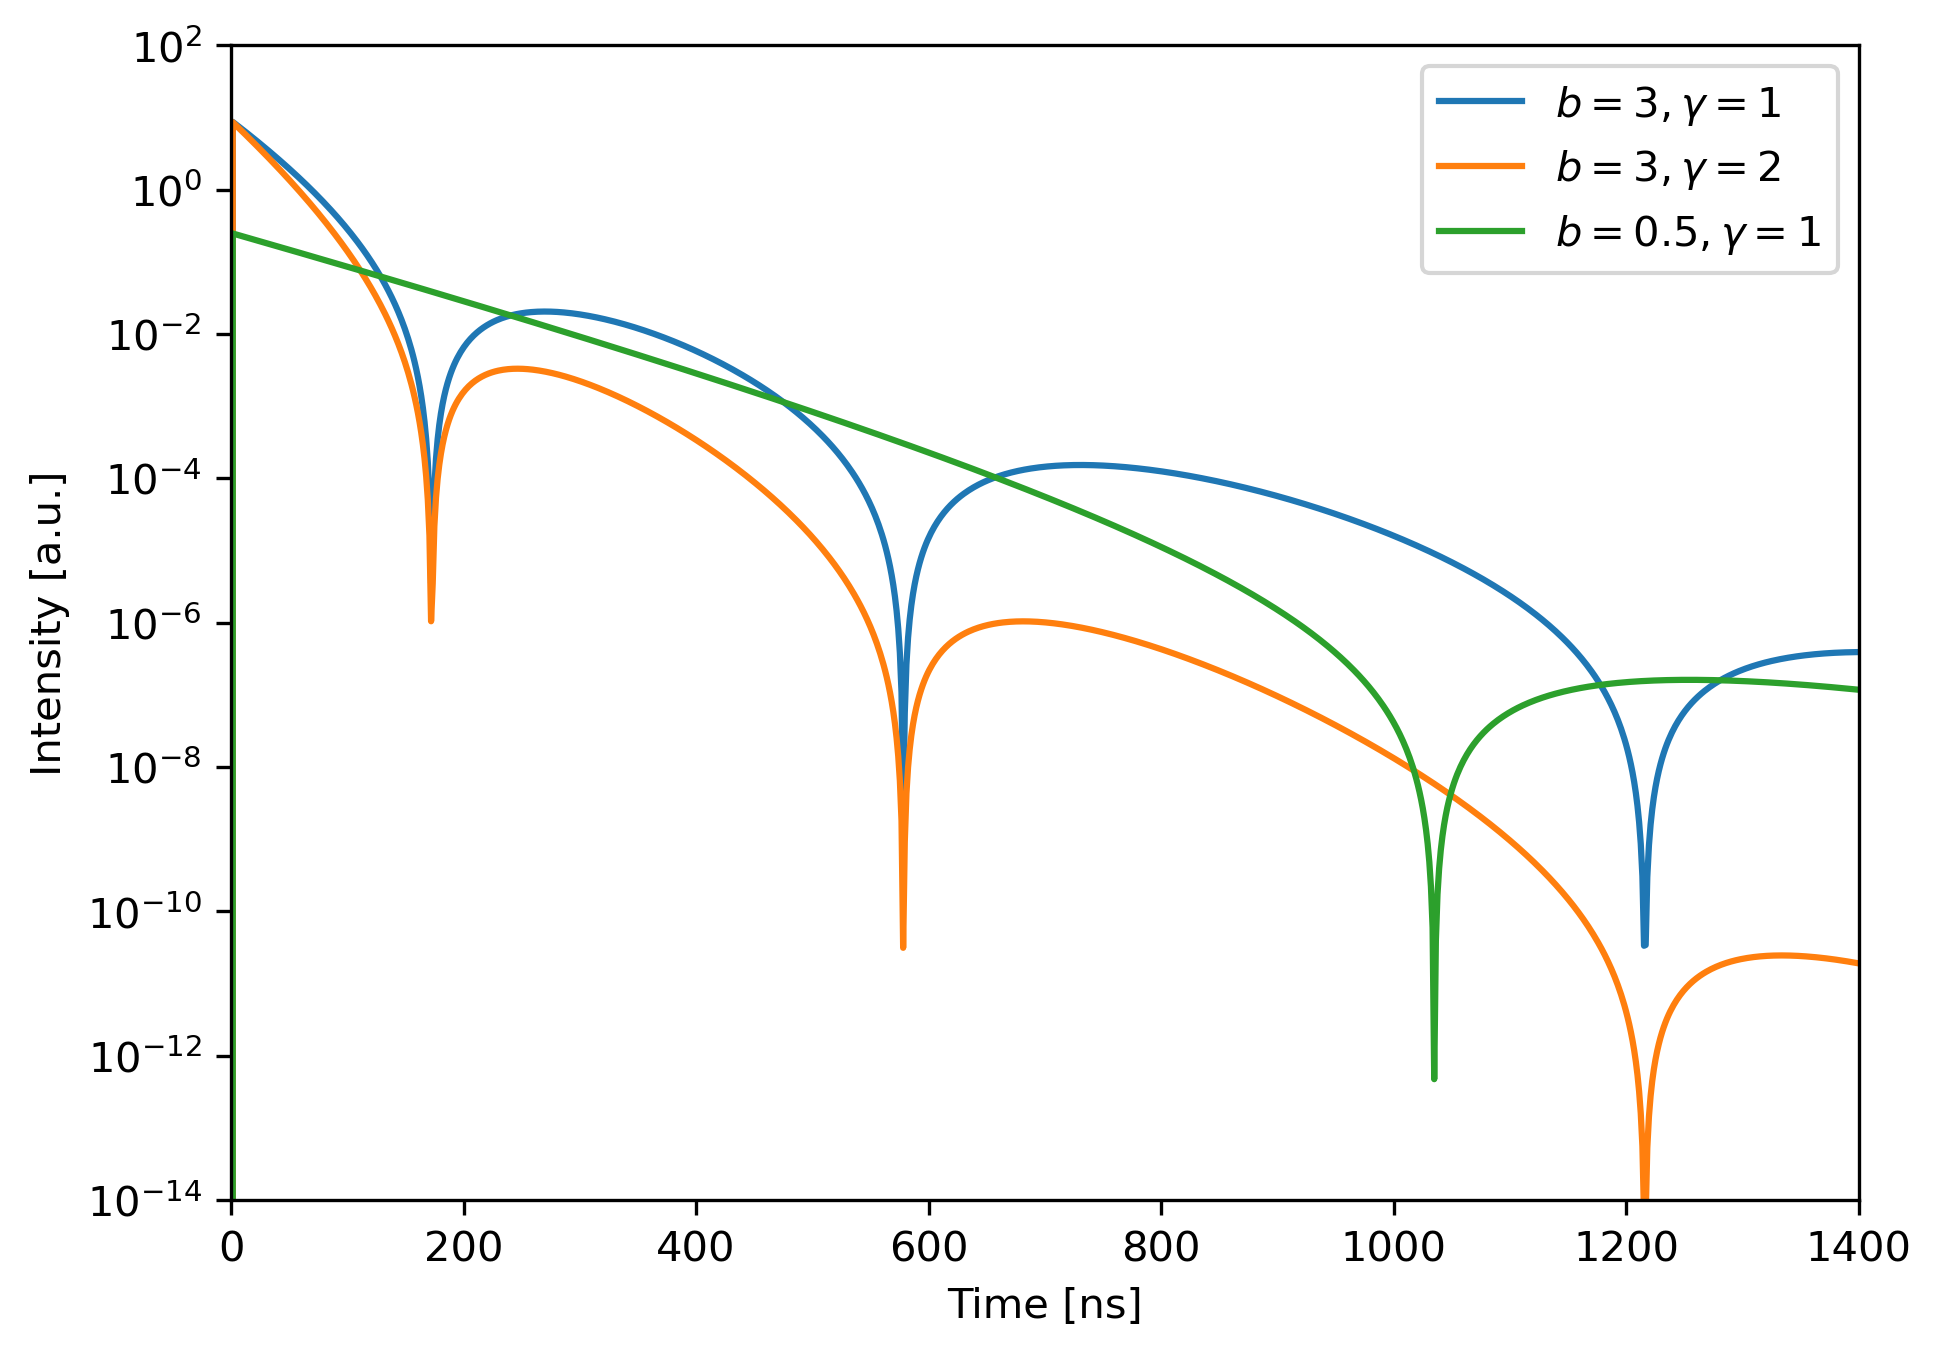
\includegraphics[width = 0.75\textwidth]{data/background/besselbeats_2.png}
    \caption{Intensity $I = |E|^2 = |R|^2$ as function of time for two different b parameters and two different $\gamma$ values , with $\Delta = 0 $. The natural lifetime of $\ce{^{57}_{}Fe} $ $\tau = 141 \mathrm{ns} $ \cite{Rhlsberger2005}, where $\gamma = 1/\tau$. Generally $\gamma^{-1} $ is used as the time scale as a dimensionless unit. For this plot, the time scale is given in nanoseconds, calculated using the natural lifetime of $\ce{^{57}_{}Fe} $, to illustrate the decay process of Iron-57}
    \label{theory_besselbeats}
\end{figure}

The first part in the \Cref{responsestep1} is the unscattered light that propagates through the medium without interaction and the second part can be interpreted as the light scattered in succesion by n resonant nuclei \cite{smirnov1996nuclear}. To evaluate the second part in \cref{responsestep1},  Cauchy's residue theorem \cite{Freitag2006} 
\begin{equation}
    \oint\limits_{C} \frac{f(z)}{(z-z_0)^n} \mathrm{d}z = \frac{-2\pi i }{(n-1)!} f^{(n-1)}(z_0)\, , \label{responsestep2}
\end{equation}
where $z_0$ is the pole and C is a semicircle in the lower/upper half plane is used. The second part in \Cref{responsestep1} has a pole at $\omega = \omega_0 - i\gamma$ and we identify  $z \hateq \omega$, $z_0 = -\Delta -i\gamma$, $f(z) = e^{-i\omega \tau}$ and $f^n = (-i\tau )^n e^{-i\omega \tau}$. Inserting these parameters into \Cref{responsestep2}, we get
\begin{equation}
    R(t,z) = \delta(t) - \frac{b}{\sqrt{b\tau}} \sum_{n=0}^{\infty} \frac{(-1)^n}{n!(n+1)!} \left(\frac{2\sqrt{b\tau}}{2} \right)^{2n+1} \; e^{-i\omega_0 \tau} e^{-\frac{\gamma \tau}{2}} \theta(\tau) \, .
\end{equation}
Here the second part of the equation can be written as a Bessel function of first kind with order one and the response function in time space reads \cite{smirnov1996nuclear}
\begin{equation} \label{responsefunction}
    R(t,z) = \delta(\tau) - \sqrt{\frac{b}{\tau}} J_1(2\sqrt{b\tau}) e^{-i\omega_0 \tau} e^{-\frac{\gamma \tau}{2}} \theta(\tau)\, .
\end{equation}



Due to the coherence and collective interference effects, such as coherent superposition of emitted light from different nuclei, \textbf{dynamical beats} emerge as a time response. To get some intuition of the thickness parameter b and dynamical beats, the response function is plotted for different b in \Cref{theory_besselbeats}. In this plot one can see how different parameters effect the form of the Response function. The parameter $\gamma $ controls the decay rate, which can be seen from the comparison of the slopes of the green and orange curves. Another very important feature of the plot are the dips, that are dependent from the parameter b. These dips are the zero crossings of the Bessel function and are called the Dynamical beats or also the \textbf{Bessel beats}. This is a multiple scattering phenomena, which arises from coherent interference of emitted light from different nuclei at different points in the target. An important characteristic of dynamical beats is, that if the target is thicker, the beats arise on shorter time scales and vice versa.

\begin{figure}
    \centering
    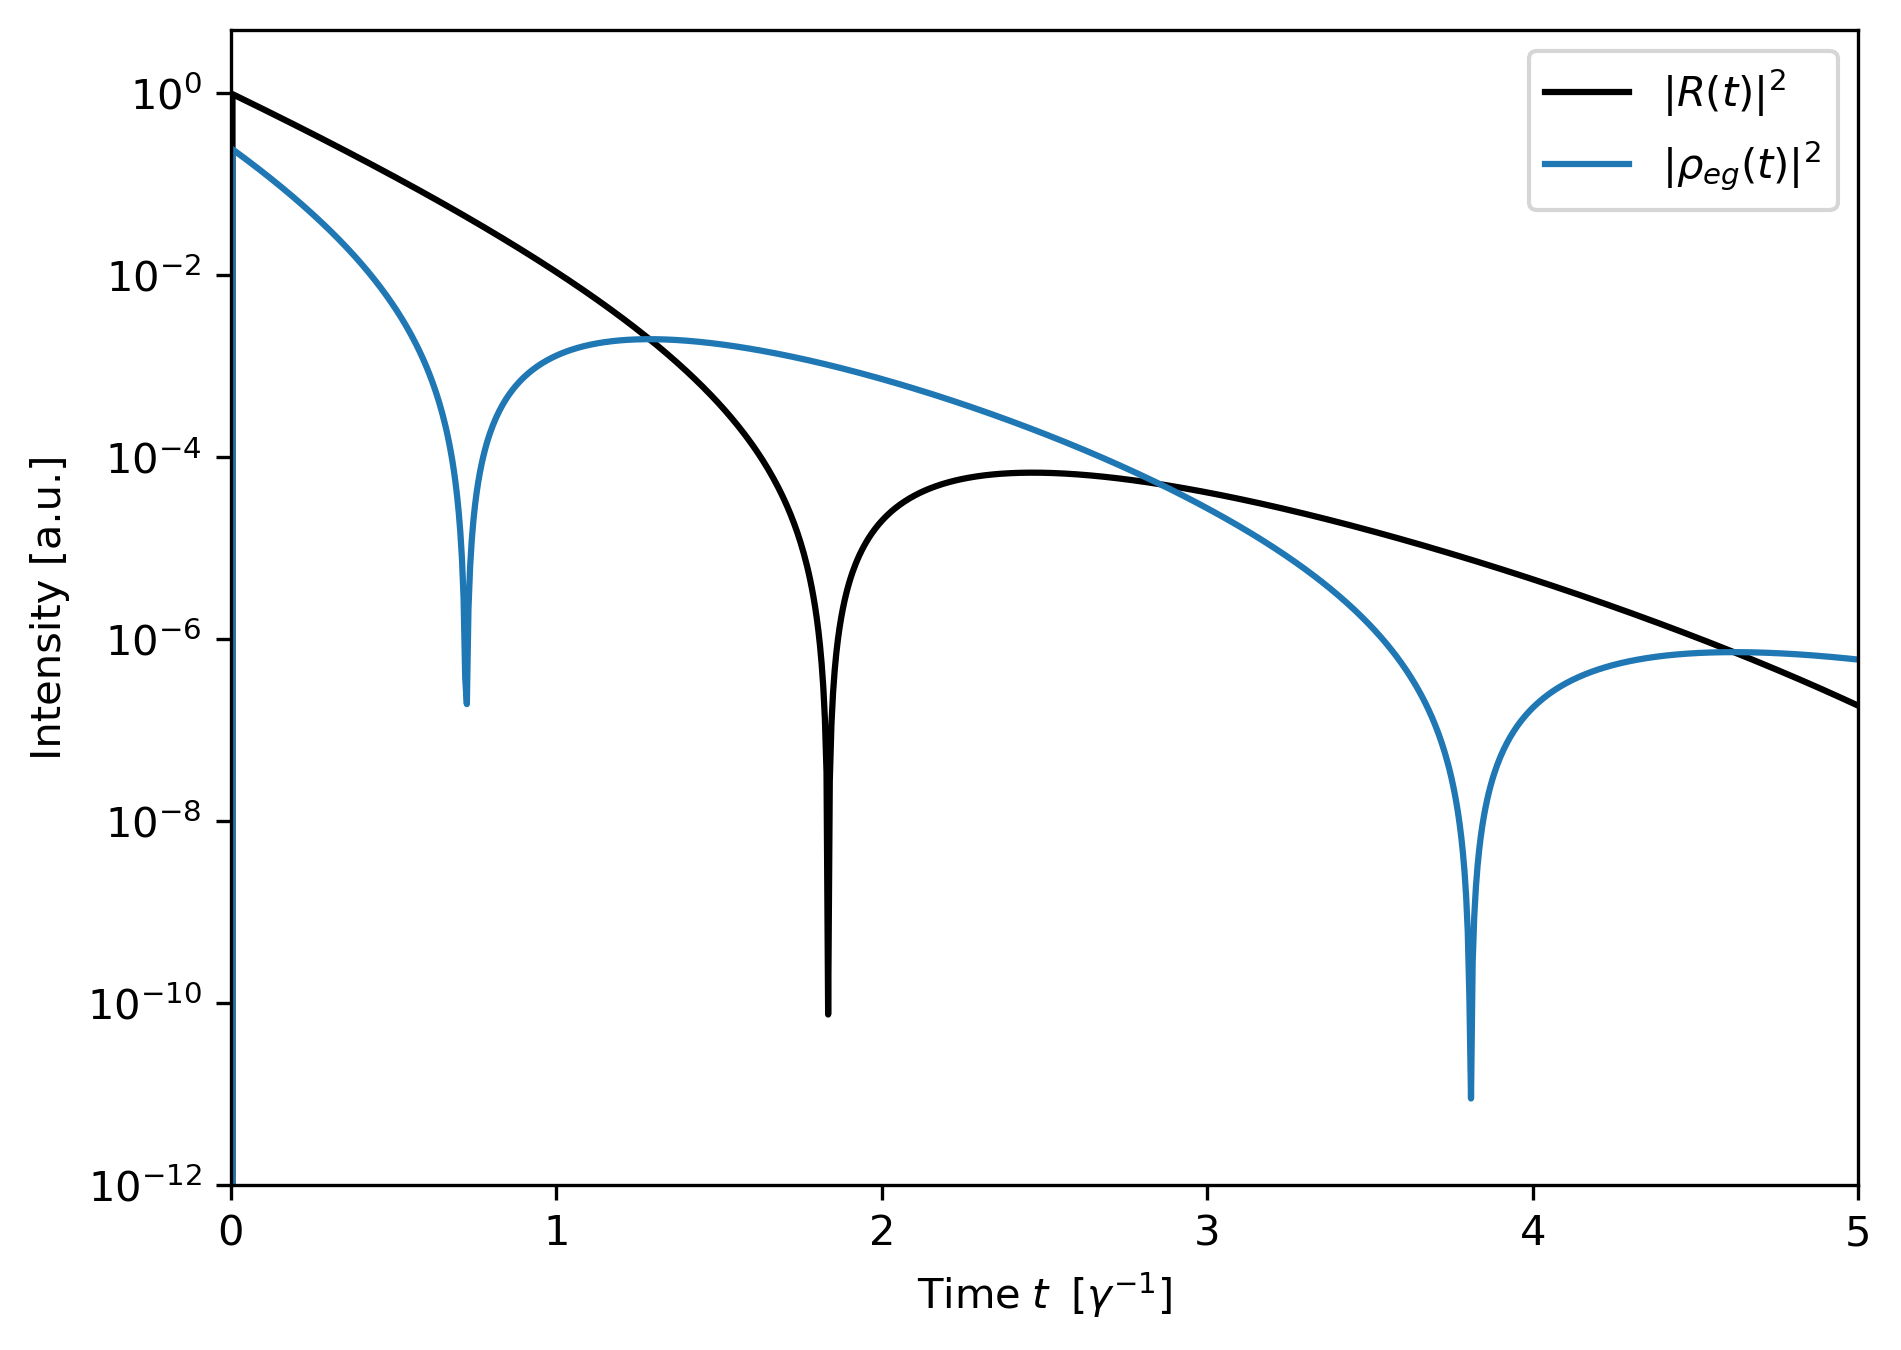
\includegraphics[width = 0.75\textwidth]{data/background/J_0__J_1_2.png}
    \caption{Response function  $I = |E|^2 = |R|^2$ in \Cref{responsefunction}  and $|\rho_{eg}|^2$ in \Cref{rhoegana} as a function of time, with $b=1$, $\Delta = 0$, $\gamma = 1$. The black curve is the time response and the blue curve is proportional to dipole moments of the target}
    \label{theory_J0J1}
\end{figure} 

\subsection{Calculation of $\rho_{eg}$ in time domain}
\Cref{timeomegapre} and \Cref{timerhoegpre} can be solved for $\Tilde{\rho}_{eg}$ instead of $\Omega$ by following the same calculation. As a result, $\Tilde{\rho}_{eg}$ is described by a Bessel function of order 0 in the time domain
\begin{equation}
    \Tilde{\rho}_{eg} = \frac{i}{2} e^{\tau (i\Delta - \frac{\gamma}{2})} J_0(2\sqrt{b\tau}) \, . \label{rhoegana}
\end{equation}

The most important difference between $\Tilde{\rho}_{eg}$ and the response function is the orders of the Bessel functions. $\rho_{eg}$ is governed by Bessel function of order 0 whereas response function by bessel function of order 1. This result agrees with the result from \cite{Smirnov1999}, where the calculated nucleus response is also described with a bessel function of order zero. Here an important relation between the first and zeroth order bessel function can be found in \cite{Smirnov1999}
\begin{equation}
    J_1(x) = -J_0^\prime(x)\, .
\end{equation}
This purely mathematical relation can be used to interpret the physical foundations of the system.\\

In the \Cref{theory_J0J1}, the difference between the response function and $\rho_{eg}$ can be seen. The Bessel beats of the $\rho_{eg}$ are coming in a much shorter time span compared to the ones of the outgoing light field. Here an important relation between $\rho_{eg}$ and the induced dipole moments is that they are proportional to each other. This can be shown by calculating the expectation value of the dipole operator, which is given as \cite{Scully_Zubairy_1997}
\begin{equation}
    \langle \hat{d}\rangle= d \, \langle\hat{\sigma}^{+}\rangle + \, h.c. \, ,
\end{equation}
where the $\hat{d}$ is the dipole-moment operator, $d$ is the dipole moment constant and the operators $\hat{\sigma}^{\pm}$ are the ladder operators, defined in \cref{lindbladian}. The expectation value for ladder operators are defined as $ \langle\hat{\sigma}^{\pm}\rangle  = tr(\hat{\rho} \cdot \hat{\sigma}^{\pm})$. We can calculate the expectation value for $\langle\hat{\sigma}^{+}\rangle $, where the $\hat{\sigma}^{+}$ is given as $\hat{\sigma}^{+} = \ket{e} \bra{g} $
\begin{align}
    \langle\hat{\sigma}^{+}\rangle  &= tr(\hat{\rho} \cdot \hat{\sigma}^{+})\\
    &=\bra{g} \hat{\rho} \cdot \hat{\sigma}^+\ket{g} + \bra{e} \hat{\rho} \cdot \hat{\sigma}^+\ket{e}\\
    &= \bra{g} \hat{\rho}\ket{e} = \rho_{ge}
\end{align}
 
\section{Burnham-Chiao Ringing}\label{section:burnhamchiao} 
Going beyond the low-excitation regime, it is no longer possible to obtain an analytical solution for the Maxwell-Bloch equations. Only under certain conditions, it is possible to obtain a solution. In the paper \cite{BURNHAM1969}, Burnham and Chiao were able to approximate the light propagation and nuclear dynamics in an excitation regime from LER to population inversion. They used two main assumptions:
\begin{enumerate}
    \item They considered only times short compared to the characteristic decay times, so we assume that $\gamma= 0$.
    \item They assumed that the medium is short enough, so that the incident pulse appears identical to each atom in the sample.
\end{enumerate}

Furthermore they modelled the atoms of the medium as harmonic oscillators, which is not valid in the inversion limit. They derived the propagation equations by integrating the harmonic oscillator into the Maxwell equations. For more detail, see eq. (3)-(4) in \cite{BURNHAM1969}. 
\subsection{Response function in low excitation regime}
In LER, they arrive to this coupled set of PDEs
\begin{subequations}
\begin{align}
    \frac{\partial \mathcal{X}(t,z)}{\partial t} &= \frac{-i f^{1/2} e}{2m \omega_0} \mathcal{E}(t,z)\label{burnham_1} \\
    \left(\frac{\partial}{\partial z} + \frac{1}{c} \frac{\partial}{\partial t}  \right) \mathcal{E}(t,z) &=  \frac{-i 2\pi f^{1/2}N e\omega_0}{c}  \mathcal{X}(t,z)\, .\label{burnham_2}
\end{align}
\end{subequations}
Here they denote $\mathcal{X}(t,z)$ as electronic displacement which can be seen as polarization and is proportional to $\rho_{eg}$, and $\mathcal{E}(t,z)$ is the electric field. Also $f$ denotes the oscillator strength, $e$ is the electronic charge, $m$ is the electronic mass, $\omega_0$ is the frequency of the harmonic oscillator and $c$ is the speed of light.\\

Using a coordination transformation $\tau = t -z/c$ and further using these substitutions
\begin{equation}
    \mathcal{X}(\tau, z) = Y(q) \;\;\; , \;\;\; Y(0) = \mathcal{X}_0\, ,
\end{equation}
where they defined $q = 2\sqrt{Q\tau z}$. They then arrive at the differential equation
\begin{equation}
    Y^{\prime \prime} + Y^\prime/q + Y = 0\, .\label{burnham_diff}
\end{equation}
The solution of this differential equation is a Bessel function of order zero and is given as follows with boundary conditions $Y(0) = \mathcal{X}_0$ and $Y^\prime (0) = 0$ for a sample of length Z and a new substitution $\tau_R = 4c/\omega_p^2 Z$, as the radiation time
\begin{subequations}
\begin{align}
    \mathcal{X}(\tau) &= \mathcal{X}_0 J_0(2\sqrt{\tau/\tau_R})\, , \label{burnham_sol1}\\
    \mathcal{E}(\tau) &= - \mathcal{E}_1 \frac{J_1(2\sqrt{\tau/\tau_R})}{\sqrt{\tau/\tau_R}}\, .
\end{align}
\end{subequations}
Here we recover the known results from our calculation in \Cref{section_respfunction}, where nucleus response $\rho_{eg}$ is governed by the Bessel function of order zero $J_0$ and the electric field by a Bessel function of order one $J_1$. 
\subsection{Beyond LER}
Going beyond the low excitation regime, in \cite{BURNHAM1969}, they introduce a vector \textbf{P} for the the two level system, where they define the angle of excitation $\Theta$ as the angle between \textbf{P} and the ground state. Doing so, the electronic displacement becomes $\mathcal{X} = P \sin{\Theta}$. Here it is good to emphasize, that they recover the \cref{burnham_1} and \cref{burnham_2} in the linear excitation regime $\Theta \approx \sin{\Theta}$. Inserting this electronic displacement equation into the propagation equations, they arrive to a sinus dependent differential equation instead of \Cref{burnham_diff}
\begin{equation}
    Y^{\prime \prime} + Y^\prime/q + \sin Y = 0\, \label{bunrhma_diff2}\, ,
\end{equation}
with the boundary conditions $Y(0) = \Theta_0$ and $Y^\prime(0) = 0$, where the excitation angle is defined in $0 \le \Theta_0 \le \pi $. This differential equation in \ref{bunrhma_diff2} is no longer analytically solvable. In the next chapters we will further investigate this paper and compare it with our results. 
\chapter{Numerical Implementation}

\section{Method of lines}
In general the optical Bloch
\chapter{Non Linear Excitation limit}
\section{Motivation}
M\"ossbauer nuclei have a very narrow spectral linewidth. 


%\chapter{Phase Scrambling}

\lipsum[7]



\chapter{Summary and outlook}

In this thesis, we aimed to analyze 



%\appendix
%\chapter{Calculation of $\rho_{eg}$ in time domain}

CALCULATION OF RHOEG 
\vspace{2cm}
CALCULATION OF RHOEG 
\vspace{2cm}
CALCULATION OF RHOEG 
%\chapter{The Table of weights for finite difference}
Here in the table given are the coefficients for the 4'th order in (\ref{fourth_order}) calculated for different offsets according to the section $\ref{weight_section}$. The Equations and their corresponding indexing for different i's look like this, where i runs from $i =0...N$:
\begin{align}
    i = 1\;\;\;\;\;&|\;\;\;\;\; \Omega_1 \approx  a_1\; \Omega_1 + a_2 \;\Omega_2 + a_3 \;\Omega_3 + \Omega_4 \;a_4 + \Omega_5\; a_5\\
    i = 2\;\;\;\;\;&|\;\;\;\;\; \Omega_2 \approx  a_1\; \Omega_1 + a_2 \;\Omega_2 + a_3\; \Omega_3 + \Omega_4 \;a_4 + \Omega_5 \;a_5\\
    [i=3] - [i = (N-2)]\;\;\;\;\;&|\;\;\;\;\; \Omega_i \approx  a_1\; \Omega_{i-2} + a_2\; \Omega_{i-1} + a_3\; \Omega_i +a_4 \; \Omega_{i+1} + a_5 \;\Omega_{i+2} \\
    i = (N-1)\;\;\;\;\;&|\;\;\;\;\; \Omega_{N-1} \approx  a_1\; \Omega_{N-4} + a_2\; \Omega_{N-3} + a_3\; \Omega_{N-2} +a_4 \; \Omega_{N-1} + a_5 \;\Omega_{N} \\
    i = N\;\;\;\;\;&|\;\;\;\;\; \Omega_{N-1} \approx  a_1\; \Omega_{N-4} + a_2\; \Omega_{N-3} + a_3\; \Omega_{N-2} +a_4 \; \Omega_{N-1} + a_5 \;\Omega_{N} \\
\end{align}


\begin{table}[h!]
    \centering
    \begin{tabular}{c|c|c|c|c|c}
$\mathbf{i}$    & $a_0$ & $a_1$ & $a_2$ & $a_3$ & $a_4$    \\ \hline
      $1$       &  -25/12& 4& -3& 4/3& -1/4 \\ \hline
      $2$       &  -1/4& -5/6& 3/2& -1/2& 1/12\\ \hline
      $3-(N-2)$ &  1/12&-2/3& 0&2/3& -1/12  \\ \hline
      $N-1$     &   -1/12& 1/2& -3/2& 5/6& 1/4\\ \hline
      $N$       &  1/4& -4/3& 3& -4& 25/12\\ \hline
      
    \end{tabular}
    \caption{Weighted Coefficients for the finite difference formula for equation (\ref{fourth_order}), calculated as demonstrated in section \ref{weight_section}. }
    \label{coefficient_table}
\end{table}

\bookmarksetup{startatroot}
\printbibliography
%\listoffigures
%\listoftables



%\chapter*{Acknowledgements}

I want to thank all my colleagues at the Max Planck Institute for the wonderful times they have created over the last six months. Especially, I want to thank my office colleagues—Miriam Gerharz, Lukas Wolff, and Robert Horn—for the fruitful discussions, the casual chess games after lunch, and the occasional Turkish lessons. I also want to thank the group and Ze-an Peng for the joyful lunch talks.\\

Another thank you goes to Lukas for discussing his results with me and answering my questions, even when he was in a hurry to catch the bus in five minutes.\\

I also want to thank Miriam for co-supervising this thesis, patiently answering all my questions about programming and physics, and proofreading this thesis. And, of course, for helping me get started with Julia!\\

Last but not least, a very special thank you goes to Jörg Evers for welcoming me into his group and showing me how to do science from scratch. Without his guidance, this thesis would not have been possible. I am also very grateful for the opportunity to attend the DPG Meeting in Freiburg and present a poster for the first time in my life!\\

Bu tez aslında liseden sonra Almanya'da geçirdiğim ilk 4 yılın bitişini de simgeliyor ve bu noktada 'ekip'i anmazsam olmaz: Sarp, Sıla, Kaan, Beste ve Ceren. Acısıyla tatlısıyla son 4 yılda çok güzel vakitler geçirdik. Sickingenstrasse 23'ü de tepe tepe kullandık valla. Daha nice beraber yıllara.\\

Ve tabii ki sevgili annem ve babam. Maddi ve manevi her zaman arkamda olduğunuzu bilmek bana güç veriyor. Iyi ki varsınız!


 
\end{document}


% \pagenumbering{roman}
% \begin{document}
	
% %% title pages similar to providet template instead of maketitle
% \subfile{titlepage} 

% \cleardoublepage

% \subfile{abstracts}
% %%%% Abstract page
%% =============
%%
%% Content of abstract pages has been put into seperate pages to simplify
%% word counting. Use e.g. the unix command
%%   wc abstract-ger.tex
%% or
%%   wc abstract-eng.tex
%% to get the number of words contained in these files.
\thispagestyle{empty}
%\begin{center}
  \noindent\sffamily\textbf{Abstract}
	\\[1em]\normalfont\normalsize

With the increasing number of nuclear-resonant photons per pulse at x-ray free electron lasers (XFELs) \cite{scientific_opp_XFEL}, achieving higher excitation levels experimentally becomes feasible \cite{Shvydko2023}. This development makes it particularly compelling to investigate light propagation and dynamics beyond the low-excitation regime (LER) and around population inversion. Thus, in this thesis, we examine the time response of resonant nuclear scattering of x-rays beyond the LER. In the LER, it is possible to obtain an analytical solution for light propagation, which becomes not possible beyond this regime. To study dynamics beyond the LER, we employ numerical methods to analyze propagation effects and nuclear dynamics. We implement the method of lines (MOL) to solve the Maxwell-Bloch equations.\\

First, we compare our results with those of Wolff \cite{wolff2023characterization} in the LER using thin targets, where the effects arising from the propagation of light through the target can be neglected. We generalize their results by analyzing the dynamics in thick targets, considering the propagation effects. Subsequently, we extend our investigation beyond the LER to the regime of population inversion and beyond. Here, we discover interesting phenomena, such as time shifts in the minima of the observed coherently scattered light intensity and transitions around population inversions. We propose an experimental signature to detect nonlinear excitations by calculating the relative time shifts as a function of target thickness. Finally, we analyze our model in the non-decaying limit ($\gamma = 0$) and find good agreement with the results from Burnham and Chiao \cite{BURNHAM1969}, concluding that spontaneous decay plays a major role in the creation of transitions around population inversions.


  \vfill
  \vspace{1cm}
  %\begin{minipage}[c][0.48\textheight][b]{0.9\textwidth}
    %\small
    %\textbf{
    %  
    %}\par
    %\vspace{\baselineskip}
    %\normalfont\normalsize
    \noindent\sffamily\textbf{Abstrakt}
	\\[1em]\normalfont\normalsize
Mit der zunehmenden Anzahl von nuklear-resonanten Photonen pro Puls beim XFELs \cite{scientific_opp_XFEL} wird es experimentell möglich, höhere Anregungsniveaus zu erreichen \cite{Shvydko2023}. Diese Entwicklung macht es besonders interessant, die Lichtausbreitung und Dynamik über das Niedriganregungsregime (LER) hinaus sowie um die Populationsinversion zu untersuchen. In dieser Arbeit analysieren wir daher das Zeitverhalten der resonanten nuklearen Streuung von Röntgenstrahlen außerhalb des LER. Im LER ist es möglich, eine analytische Lösung für die Lichtausbreitung zu erhalten, was in höheren Anregungsbereichen nicht mehr möglich ist. Um die Dynamik in diesen höheren Bereichen zu untersuchen, verwenden wir numerische Methoden, um die Ausbreitungseffekte und die Kerndynamik zu analysieren. Wir implementieren die Methode der Linien (MOL), um die Maxwell-Bloch-Gleichungen zu lösen.\\

Zunächst vergleichen wir unsere Ergebnisse mit denen von Wolff \cite{wolff2023characterization} im LER unter Verwendung dünner Targets, bei denen die durch die Lichtausbreitung im Target entstehenden Effekte vernachlässigt werden können. Wir erweitern deren Ergebnisse, indem wir die Dynamik in dicken Targets unter Berücksichtigung der Ausbreitungseffekte analysieren. Anschließend untersuchen wir den Bereich der Populationsinversion und darüber hinaus. Hier entdecken wir interessante Phänomene wie Zeitverschiebungen in den Minima der beobachteten kohärent gestreuten Lichtintensität und Übergänge um die Populationsinversionen. Wir schlagen eine experimentelle Signatur vor, um nichtlineare Anregungen durch Berechnung der relativen Zeitverschiebungen in Abhängigkeit von der Targetdicke zu detektieren. Schließlich analysieren wir unser Modell im nicht zerfallenden Grenzfall ($\gamma = 0$) und finden eine gute Übereinstimmung mit den Ergebnissen von Burnham und Chiao \cite{BURNHAM1969}. Wir kommen zu dem Schluss, dass der spontane Zerfall eine wesentliche Rolle bei der Entstehung der Übergänge um die Populationsinversionen spielt.
    %\input{abstract-eng}
  %\end{minipage}
%\end{center}


% \tableofcontents

% \cleardoublepage

% \pagenumbering{arabic}

% %% Put your contents here
% \subfile{chap_intro}
% \subfile{chap_background}
% \subfile{chap_phasescramb}
% \subfile{chap_highlow}


% \renewcommand\thepart{}
% \renewcommand\partname{}
% \part{Appendices}
% \setcounter{part}{0}
  
% \appendix
% \subfile{chap_appendixA}
% \subfile{chap_appendixB}
%   	%%%\subfile{content/99_Appendices/x_TODOS}
  
% %\chapter{Lists}


% %    
% \bookmarksetup{startatroot}
% \printbibliography
% %    \include{deposition}

% \cleardoublepage

% \subfile{chap_acknowledge}

	
% \end{document}
